
\definecolor{verde}{rgb}{0.25,0.5,0.35}
\definecolor{jpurple}{rgb}{0.5,0,0.35}
\definecolor{darkgreen}{rgb}{0.0, 0.2, 0.13}




\newcommand{\estiloR}{
	\lstset{ %
		language=R,                     % the language of the code
		basicstyle=\footnotesize,       % the size of the fonts that are used for the code
		numbers=left,                   % where to put the line-numbers
		numberstyle=\tiny\color{gray},  % the style that is used for the line-numbers
		stepnumber=1,                   % the step between two line-numbers. If it's 1, each line
		% will be numbered
		numbersep=5pt,                  % how far the line-numbers are from the code
		backgroundcolor=\color{white},  % choose the background color. You must add \usepackage{color}
		showspaces=false,               % show spaces adding particular underscores
		showstringspaces=false,         % underline spaces within strings
		showtabs=false,                 % show tabs within strings adding particular underscores
		frame=single,                   % adds a frame around the code
		rulecolor=\color{black},        % if not set, the frame-color may be changed on line-breaks within not-black text (e.g. commens (green here))
		tabsize=2,                      % sets default tabsize to 2 spaces
		captionpos=b,                   % sets the caption-position to bottom
		breaklines=true,                % sets automatic line breaking
		breakatwhitespace=false,        % sets if automatic breaks should only happen at whitespace
		title=\lstname,                 % show the filename of files included with \lstinputlisting;
		% also try caption instead of title
		keywordstyle=\color{blue},      % keyword style
		commentstyle=\color{darkgreen},   % comment style
		stringstyle=\color{red},      % string literal style
		escapeinside={\%*}{*)},         % if you want to add a comment within your code
		morekeywords={*,...}          % if you want to add more keywords to the set
}}

\definecolor{aliceblue}{rgb}{0.94, 0.97, 1.0}


\chapter{Geoestatística utilizando o software R}


\section{Introdução}

A geoestatística é uma ciência que envolve a manipulação de dados, o que torna imprescindível o uso de programação e softwares. A programação em R é uma linguagem aplicada especificamente para análise estatística computacional e geração de gráficos. Além de possuir uma quantidade grande de bibliotecas que podem ser utilizadas facilmente, existe um grande aporte da comunidade no desenvolvimento e manutenção de novas rotinas. 

O R é uma linguagem de programação, e por meio de linhas de comando é possível gerar um algoritmo que permita a análise estatística dos dados fornecidos. Para os inciantes na programação, podemos pensar no algoritmo como uma sequência de instruções a ser realizada para o cumprimento de uma tarefa. Programar, nada mais é, que interagir com  o computador, e permitir com que ele faça as tarefas de acordo com suas ordens. Imagine que precisemos fabricar um bolo de chocolate. Para realizarmos estas tarefas realizamos os seguintes passos: 


\vspace{0.5cm}
\colorbox{aliceblue}{\begin{minipage}{\textwidth}
\textbf{Algoritmo para a fabricação de um bolo} 
\begin{enumerate}
	\item Compramos os ingredientes 
	\item Retiramos os vasilhames da dispensa 
	\item Misturamos a massa 
	\item Fabricamos a cobertura 
	\item Assamos o bolo 
	\item Cobrimos o bolo com a cobertura
\end{enumerate} 
\end{minipage}}
\vspace{0.5cm}


Note que para fabricarmos um bolo precisamos seguir a ordem das instruções, pois não podemos misturar a massa antes de comprar os ingredientes, por exemplo. Essa ordem de predecessão é necessária para que a atividade se cumpra. 

No entanto, podemos adicionar estruturas neste algoritmo para que ele se adapte a diferentes condições. Imagine que já tenhamos uma quantidade de ingredientes já comprados. Devemos verificar na dispensa se existe este ingrediente primeiro. Isso pode ser realizado como uma estrutura condicional. O algoritmo se transformaria em: 


\vspace{0.5cm}
\colorbox{aliceblue}{\begin{minipage}{\textwidth}
\textbf{Algoritmo para a fabricação de um bolo} 
\begin{enumerate}
	\item Se ingredientes estão na dispensa 
	\subitem Não comprar ingredientes
	\item Senão 
	\subitem comprar ingredientes
	\item Retiramos os vasilhames da dispensa 
	\item Misturamos a massa 
	\item Fabricamos a cobertura 
	\item Assamos o bolo 
	\item Cobrimos o bolo com a cobertura
\end{enumerate} 
\end{minipage}}
\vspace{0.5cm}


Muita vezes também é necessário realizar tarefas repetitivas, e se torna necessário resumir um número grande de instruções. Neste casso utilizamos estruturas de repetição. Se quiséssemos montar uma fábrica de bolo, poderíamos realizar o seguinte algoritmo:

\vspace{0.5cm}
\colorbox{aliceblue}{\begin{minipage}{\textwidth}	
\textbf{Algoritmo para a fabricação de um bolo}
\begin{enumerate}
	\item Compramos os ingredientes
	\item Retiramos os vasilhames da dispensa  
	\item Enquanto houver ingredientes faça
	\subitem Misturamos a massa 
	\subitem Fabricamos a cobertura 
	\subitem Assamos o bolo 
	\subitem Cobrimos o bolo com a cobertura
\end{enumerate} 
\end{minipage}}
\vspace{0.5cm}

Apesar de simples, a fabricação de um bolo ilustra de forma intuitiva o que significa um algoritmo. Para fins de comunicação com uma máquina, se torna necessário o uso de uma linguagem de programação, que permitirá "falar" as instruções para o computador de forma efetiva. No entanto, computadores comunicam apenas com valores binários de 0 e 1. Quanto mais próxima é uma linguagem em comunicar com o computador neste patamar, chamamos esta linguagem de baixo nível. No entanto, quanto mais a linguagem de computação for próxima da linguagem convencional que nós humanos utilizamos, chamamos esta linguagem de alto nível. O R é uma linguagem de alto nível que permite comunicarmos com o computador a partir de instruções praticamente como a escrita em inglês.

Nas próximas seções verificaremos como utilizar um algoritmo e a linguagem R, e como aplicar as funções necessárias para realizar geoestatística em um depósito mineral simples. Utilizaremos o depósito fictício Walker Lake, demonstrado no livro dos professor Issac e Srivastava \cite{isaaks1989applied}. Este depósito foi construído a partir de medidas topográficas de uma região em Nevada, no Canadá. As variáveis trabalhadas correspondem a medidas imaginárias V e U.

\section{Instalação do R}

Para utilizar o R precisamos inicialmente instalar o pacote do site \url{https://www.r-project.org/}. Para  utilizar a linguagem é recomendado o uso de uma IDE (Integrated Development Enviroment) de programação. Recomendamos utilizar o RStudio como plataforma para desenvolver os algoritmos. O software pode ser baixado no site \url{https://www.rstudio.com/}. 

\section{RStudio} 

O RStudio é uma IDE (Integrated Development Enviroment) gratuita para análise de algoritmos em R. A figura \ref{RStudio} demonstra as janelas do aplicativo utilizada para as análises estatísticas. No editor é possível criarmos rotinas, escrevendo todas as instruções desejadas e selecionando as desejadas para serem aplicadas. Na janela de variáveis de ambiente observamos todas as variáveis criadas, seu tipo e valores. No console podemos aplicar instruções individualmente, atuando uma instrução de cada vez. E finalmente na janela de output são demonstrados os gráficos, arquivos gerados e pacotes habilitados pelo programa. 

\FloatBarrier
\begin{figure}[H]
	\centering
	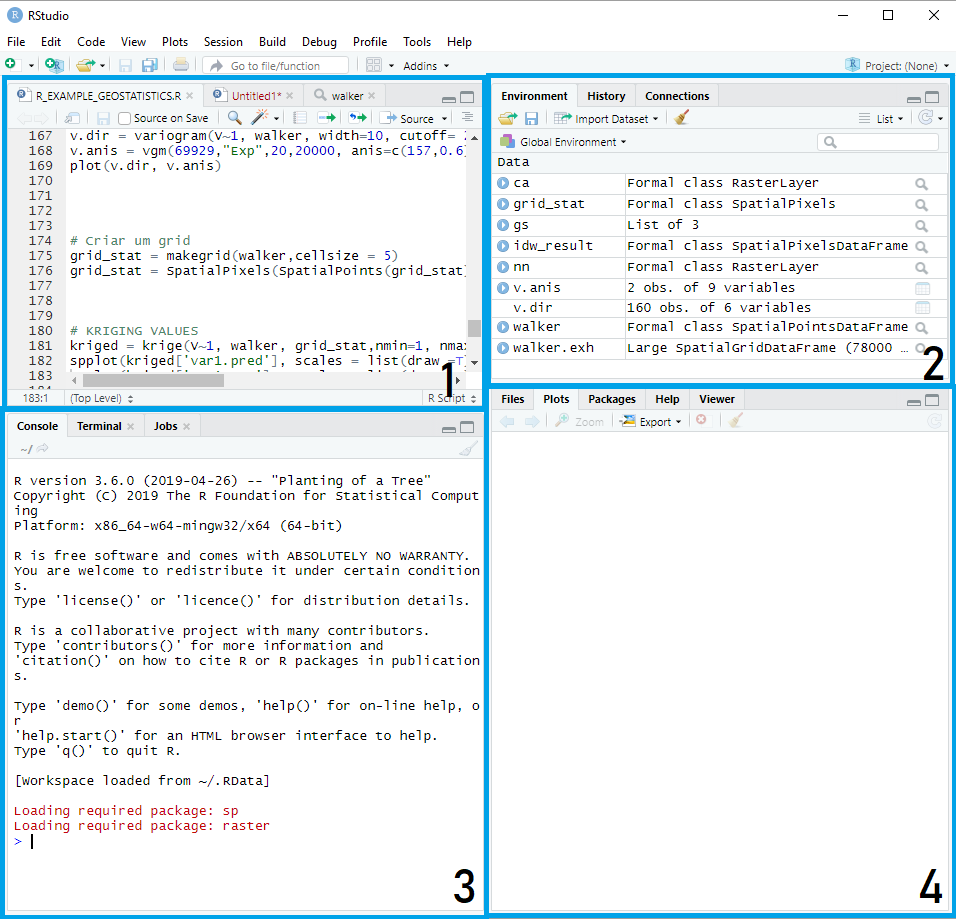
\includegraphics[scale=0.6]{R_studio.png}	
	\caption{Demonstração da janela do RStudio. 1 - Editor,  2-Variáveis de ambiente, 3-Console, 4- Output}
	\label{RStudio}
\end{figure}
\FloatBarrier


\section{Noções preliminares}

Muitas vezes desejamos deixar lembretes no nosso código para que futuramente possamos entender melhor as instruções utilizadas. Para realizar comentários no código, utilizamos o símbolo \# e em seguida escrevemos o que desejamos na frente do símbolo.  Outro importante operador é o de atribuição -> ou =. Este é responsável por associar um valor a uma variável. Uma variável é um objeto capaz de guardar na memória um certo valor, por exemplo um número, um texto, ou até mesmo outro objeto. 

\begin{scriptsize}
	\estiloR
	\begin{lstlisting}[]
	
	nome = "David"                 # Atribui um texto na variavel nome
	numero = 45.6                  # Atribui um numero na variavel
	grafico = hist(dados$V)        # Atribui um objeto na variavel
	
	\end{lstlisting}
\end{scriptsize}
 
 Em alguns casos podemos atribuir uma variável a ela mesma. Lembre-se que o operador = não significa igualdade, mas atribuição. O exemplo abaixo demonstra este resultado. 
 
 \begin{scriptsize}
 	\estiloR
 	\begin{lstlisting}[]
 	
 	numero = 5 						# Atribui 5 na variavel 
 	numero = numero + 1				# Adiciona um na variavel 5, retornando 6
 	
 	\end{lstlisting}
 \end{scriptsize}

\section{O R como uma calculadora}

Assim como uma calculadora comum o R realiza cálculos básicos como subtração, adição, subtração, soma, etc. Deve-se lembrar sempre da predecessão dos operadores matemáticos no momento de realizar os cálculos, podendo ser utilizados parênteses para definir as relações de cálculo.  

\begin{scriptsize}
	\estiloR
	\begin{lstlisting}[]
		
	2+2 # Soma            
	2-2 # Subtracao      
	2*2 # Multiplicacao      
	2/2 # Divisao            
	2^2 # Exponenciacao  
	7%2 # Resto da divisao    
	3*(4-3)^2        
	         
	\end{lstlisting}
\end{scriptsize}

\section{Utilizando funções no R}

Para utilizar uma função é necessário escrever seu nome e adicionar seus argumentos dentro de parênteses. Usualmente atribui-se o nome do argumento e então é atribuído seu valor. Podemos passar argumentos sem seus nomes também, e dessa forma a predecessão de cada um destes é atribuído segundo a ordem estabelecida pela função. Abaixo encontramos algumas funções comuns do R.

\begin{scriptsize}
	\estiloR
	\begin{lstlisting}[caption={Operacoes matemáticas convencionais utilizando o R}, label=lst:rcode]
	
	log(3)         # logaritmo natural de  3 
	sqrt(45)       # raiz quadrada de 45 
	factorial(4)   # fatorial de 4 , 4!
	abs(5-3)       # valor absoluto de 2  
	
	
	\end{lstlisting}
\end{scriptsize}

\section{Operadores Relacionais} 

Operadores relacionais são aqueles utilizados para comparar valores entre números ou expressões. O resultado de um operador relacional é um valor booleano que indica se a expressão é verdadeira ou falsa. Os operadores utilizados no R são demonstrado na tabela abaixo. É importante lembrar que o operador = é associado à atribuição de uma variável ao contrário do operador == que representa igualdade: 

\FloatBarrier
\begin{table}[]
	\centering
	\begin{tabular}{@{}ll@{}}
		\toprule
		Operador & Relação \\ \midrule
		== & Igualdade \\
		!= & Diferente \\
		> & Maior \\
		< & Menor \\
		>= & Maior e igual \\
		<= & Menor e igual \\ \bottomrule
	\end{tabular}
	\caption{Operadores relacionais no R}
	\label{tab:my-table}
\end{table}
\FloatBarrier

Abaixo é apresentado alguns resultados dos operadores relacionais para o R. 

\begin{scriptsize}
	\estiloR
	\begin{lstlisting}[caption={Exemplo de operadores relacionais no R}, label=lst:rcode]
	
	3 == 5         # Retorna FALSO
	5 > 3          # Retorna VERDADEIRO 
	-2 < 7         # Retorna VERDADEIRO
	abs(-5+3)== 2  # Retorna VERDADEIRO  
	4 != 4 		     # Retorna FALSO
	
	
	\end{lstlisting}
\end{scriptsize}

\section{Operadores Lógicos no R} 

A utilização de operadores booleanos na programação é algo muito comum quando precisamos avaliar relações múltiplas. A lógica matemática é o fundamento principal de um operador lógico que retorna um valor booleano (Verdadeiro ou Falos) a partir de um conjunto de relações. As operações mais comuns são o E, simbolizado por \& e o OU, simbolizado por ||. 

O operador E retorna valor verdadeiro apenas se as duas premissas relacionadas forem verdadeiras. A frase " A ferrari é uma marca de carro, E é muito cara" retorna valor verdadeiro, pois ambas são de fato verdade. A tabela verdade abaixo demonstra o resultado do operador E assumindo os valores de cada uma das premissas utilizadas. 

\FloatBarrier
\begin{table}[h]
	\centering
	\begin{tabular}{@{}lll@{}}
		\toprule
		Valor 1    & Valor 2    & Operação E \\ \midrule
		Verdadeiro & Verdadeiro & Verdadeiro \\
		Falso      & Verdadeiro & Falso      \\
		Verdadeiro & Falso      & Falso      \\
		Falso      & Falso      & Falso      \\ \bottomrule
	\end{tabular}
	\caption{Tabela verdade do operador E}
	\label{tab:my-table}
\end{table}
\FloatBarrier

Já o operador OU retorna valor falso apenas se as duas premissas relacionadas forem falsas, retornando verdadeiro em todos os outros casos. A frase "A ferrari não é uma marca de carro, OU é muito cara" retorna valor verdadeiro, pois a marca é muito cara. A tabela verdade abaixo demonstra as relações do operador OU.

\FloatBarrier
\begin{table}[h]
	\centering
	\begin{tabular}{@{}lll@{}}
		\toprule
		Valor 1    & Valor 2    & Operação OU \\ \midrule
		Verdadeiro & Verdadeiro & Verdadeiro \\
		Falso      & Verdadeiro & Verdadeiro     \\
		Verdadeiro & Falso      & Verdadeiro     \\
		Falso      & Falso      & Falso      \\ \bottomrule
	\end{tabular}
	\caption{Tabela verdade do operador OU}
	\label{tab:my-table}
\end{table}
\FloatBarrier

A script abaixo demonstra operações relacionais no R

\begin{scriptsize}
	\estiloR
	\begin{lstlisting}[caption={Exemplo de operadores relacionais no R}, label=lst:rcode]
	
	(5>4) & (3<7)         # Retorna VERDADEIRO
	(5>4) & (3<2)         # Retorna FALSO 
	(7==4) || (2>3)       # Retorna FALSO
	(3>2) || (2>3)        # Retorna VERDADEIRO
	
	
	\end{lstlisting}
\end{scriptsize}

\section{Pedindo ajuda no R} 


Muitas vezes não conhecemos adequadamente o funcionamento de alguma função ou comando. Para procurar ajuda, o R possui a função help() que auxilia na identificação dos argumentos da função, ou simplesmente pode-se colocar o símbolo ? antes da função que se pretende identificar.

\begin{scriptsize}
	\estiloR
	\begin{lstlisting}[caption={Exemplo de ajuda utilizando a função help}, label=lst:rcode]
	
	help(par) # Ajuda para a funcao par 
	?par      # Ajuda para a funcao par 
	
	\end{lstlisting}
\end{scriptsize} 

\section{Pacotes do R}

Uma das grandes vantagens da utilização do R consiste em sua grande quantidade de pacotes disponíveis de todos os tipos. É necessário no R instalar estes pacotes utilizando o comando install.packages. A opção "dependences" permite com que o pacote instale qualquer outro tipo de dependência necessária para o funcionamento do pacote, assumindo valor verdadeiro = T ou TRUE, ou valor falso = F ou FALSE.  Utilizaremos neste livro dois pacotes importantes para a análise dados, o pacote sp, responsável por análises espaciais e o pacote gstat e geoR, responsáveis para realizar a análise geoestatística. 

\begin{scriptsize}
	\estiloR
	\begin{lstlisting}[caption={Código fonte em R para instalação dos pacotes necessários}, label=lst:rcode]
	
	# Comandos para instalacao dos pacotes
	install.packages(sp, dependences=T)
	install.packages(gstat, dependences =T)
	install.packages(geoR, dependences = T)
	
	# Comandos para carregar os pacotes 
	library(sp)
	library(geoR)
	library(gstat)
	\end{lstlisting}
\end{scriptsize}

\section{Criando vetores}

Vetores são objetos capazes de armazenar vários dados. É possível armazenar em vetores tanto variáveis numéricas como também textos, porém, apenas um tipo de variável deve ser adicionado em cada vetor. Para criar um vetor de dados inicia-se com a letra c, colocando os valores na ordem desejada separados de vírgula. O código abaixo demonstra  a criação de um vetor de dados. 

\begin{scriptsize}
	\estiloR
	\begin{lstlisting}[caption={Criação de um vetor em R}, label=lst:rcode]
	
	# Criacao de um vetor de numeros
	dedos = c(1,2,3,4,5,6,7,8,9,10)
	
	# Criacao de um vetor de textos
	aves = c("tucano", "gaivota", "pombo")
	
	\end{lstlisting}
\end{scriptsize}

Algumas operações podem ser realizadas com estes vetores. 

\begin{scriptsize}
	\estiloR
	\begin{lstlisting}[caption={Criação de um vetor em R}, label=lst:rcode]
	
	# Criacao de um vetor de numeros
	dedos = c(1,2,3,4,5,6,7,8,9,10)
	
	max(dedos)        # Retorna o valor maximo do vetor dedos
	min(dedos)		    # Retorna o valor minimo do vetor dedos
	sum(dedos)		    # Retorna a soma dos itens do vetor dedos
	length(dedos)     # Retorna o tamanho do vetor dedos
	
	\end{lstlisting}
\end{scriptsize}

Para acessar um valor do vetor podemos utilizar um colchetes para indicar a posição do elemento desejado. Caso deseje retornar o vetor sem um elemento podemos usar índices negativos.


\begin{scriptsize}
	\estiloR
	\begin{lstlisting}[caption={Criação de um vetor em R}, label=lst:rcode]
	
	# Criacao de um vetor de numeros
	vetor= c(5,4,12,11,45,6,7)
	
	vetor[1]           # Retorna 5
	vetor[2]    	     # Retorna 4
	vetor[-1]          # Retorna 4,12,11,45,6,7
	\end{lstlisting}
\end{scriptsize}

Podemos gerar sequências de números também utilizando os dois pontos. Por exemplo, para gerar números de um a dez podemos usar o comando 1:10. Podemos gerar sequências de números também utilizando a função seq(), para isso utilizamos os atributos from, para identificar o número de início, to, para identificar o valor final e by, para identificar o passo de um número para outro. Podemos gerar também repetições com o comando rep(). O resultado de rep(5,4) será c(5,5,5,5).

\begin{scriptsize}
	\estiloR
	\begin{lstlisting}[caption={Criação de um vetor em R}, label=lst:rcode]
	
	1:10 					                  # gera 1 2 3 4 5 6 7 8 9 10
	seq(from=1, to=10, by=2)         # gera 1 3 5 7 9
	rep(5,4)				                  # gera 5 5 5 5
	
	\end{lstlisting}
\end{scriptsize}

\section{Condicional} 

Como visto no exemplo do bolo, podemos indicar condições para o cumprimento de uma determinada tarefa. Ao utilizar o operador IF, conseguimos determinar se instruções serão realizadas ou não de acordo com uma condição. No exemplo abaixo o algoritmo verifica se o valor C é maior que 5, e em seguida o valor de C é demonstrado na tela, caso o contrário é utilizado o comando else, e demonstrado na tela o valor de 5. Para separar uma instrução condicional de outra é utilizado o colchetes.

\begin{scriptsize}
	\estiloR
	\begin{lstlisting}[caption={Criação de um vetor em R}, label=lst:rcode]
	
	
	If (C > 5){
		print(C)
	}
	else{
		print(5)
	}
	
	\end{lstlisting}
\end{scriptsize}

\section{Repetições}

Commo visto no exemplo do bolo, podemos repetir instruções de acordo com uma ordem. Um dos operadores que pode ser facilmente utilizado para repetições é o for. Outro tipo de repetição é quando utilizamos a estrutura while, em que a repetição ocorre até encontrar uma condição de parada. Muito cuidado deve-se ter ao utilizar a estrutura while, pois se a repetição não encontrar a condição de parada ela se repetirá infinitamente, consumindo a memória do computador. O exemplo abaixo plota os dez primeiros números de uma sequência fornecida utilizando tanto o comando for como while. 

\begin{scriptsize}
	\estiloR
	\begin{lstlisting}[caption={Criação de um vetor em R}, label=lst:rcode]

	for (i in 1:10){
		print(i)
	}
	
	i = 1
	while(i <= 10){
		print(i)
		i = i + 1
	}
	\end{lstlisting}
\end{scriptsize}

\section{Concatenação de funções} 

Em muitos os casos podemos concatenar funções dentro de outras funções, assim como também podemos concatenar operadores dentro de operadores. As condicionais podem ser realizadas uma dentro das outras, assim como as repetições podem ser realizadas uma dentro das outras. Veja os exemplos abaixo

\begin{scriptsize}
	\estiloR
	\begin{lstlisting}[caption={Criação de um vetor em R}, label=lst:rcode]
	
	y = sqrt(abs(-16))  # Retorna 4
	
	if (C> 5){					# Verifica a primeira condicao
		if (C/2 == 3){			# Verifica a segunda condicao
			print("ok")
		}
	}
	\end{lstlisting}
\end{scriptsize}


\section{DataFrames} 

Para trabalhar com dados é necessário organização, de forma a acessar os valores de forma rápida e eficiente. O DataFrame é um dos objetos do R responsáveis por organizar estes dados. A tabela abaixo demonstra um DataFrame para o conjunto de dados do Walker Lake. No topo temos o nome de cada coluna (ID, V, U, T), enquanto a esquerda temos o nome de cada linha, representado pelos números 1,2,3. Para acessar uma coluna do DataFrame devemos escrever o nome do dataframe, colocar um sinal de \$, em seguida o nome da variável.  

\FloatBarrier
\begin{table}[h]
	\centering
	\begin{tabular}{@{}lllll@{}}
		\toprule
		& Id & V & U & T \\ \midrule
		1 & 1 & 0.0 & NA & 2 \\
		2 & 2 & 0.0 & NA & 2 \\
		3 & 3 & 224.4 & NA & 2 \\ \bottomrule
	\end{tabular}
	\caption{Exemplo de DataFrame no R}
	\label{tab:my-table}
\end{table}
\FloatBarrier

A biblioteca sp contém em seus bancos de dados internos o depósito do Walker Lake. Para acessar estes dados basta apenas utilizar a função data(walker) e assim estará disponível a variável walker para uso. Para vizualizarmos alguns dados do banco podemos utilizar a função head() em que é mostrado as primeiras linhas dos dados. Podemos também utilizar a função tail() para verificar os últimos dados do banco. Uma função importante é a função summary, que permite realizar um resumo estatístico dos dados. 

\begin{scriptsize}
	\estiloR
	\begin{lstlisting}[caption={Criação de um vetor em R}, label=lst:rcode]
	
	# Comandos para instalacao dos pacotes
	install.packages(sp, dependences=T)
	install.packages(gstat, dependences =T)
	install.packages(geoR, dependences = T)
	
	# Comandos para carregar os pacotes 
	library(sp)
	library(geoR)
	library(gstat)
	
	data(walker)            #Baixa o conjunto de dados do Walker Lake
	head(walker)            # Observa os primeiros valores do Walker Lake
	tail(walker)            # Observa os ultimos valores do Walker Lake
	summary(walker)         # Realiza um sumario estatistico do Walker Lake
	
	\end{lstlisting}
\end{scriptsize}

No entanto, nem sempre é comum trabalharmos com dados já disponibilizados nas bibliotecas. O R possui funções para importação de dados CSV, excel e de banco de dados. Para isso podemos utilizar a função read.table() ou read.csv() para abrirmos um arquivo de texto ou csv. A função file.choose() permite com que uma janela para arquivos seja aberta, facilitando encontrar o endereço do arquivo. O argumento header verifica se o banco de dados possui um cabeçalho e o argumento sep verifica qual separador é utilizado para dividir as colunos no banco de dados. No caso de arquivos csv, o separador é a vírgula.


\begin{scriptsize}
	\estiloR
	\begin{lstlisting}[caption={Criação de um vetor em R}, label=lst:rcode]
	
	# Importacao de dados a partir de uma tabela ou arquivo csv
	dados = read.table(file.choose(), header =TRUE)
	dados = read.csv(file.choose(), header= TRUE, sep=",")
	
	\end{lstlisting}
\end{scriptsize}

\section{Mapa de localização} 

O posicionamento das amostras no mapa é de extrema importância para a análise espacial dos dados. Para realizarmos um mapa de localização das amostras podemos utilizar a biblioteca geoR, transformando o dataframe em um arquivo geodata e em seguida aplicando a função points. 

\begin{scriptsize}
	\estiloR
	\begin{lstlisting}[caption={Criação de um vetor em R}, label=lst:rcode]
	
	points(as.geodata(walker$V))
	
	\end{lstlisting}
\end{scriptsize}

O resultado do gráfico pode ser demonstrado na figura abaixo. Nota-se que o Walker Lake apresenta uma malha regular amostrada e valores agrupados em corpos específicos, um maior situado no flanco oeste e corpos menores situados no flanco leste.

\FloatBarrier
 \begin{figure}[H]
	\centering
	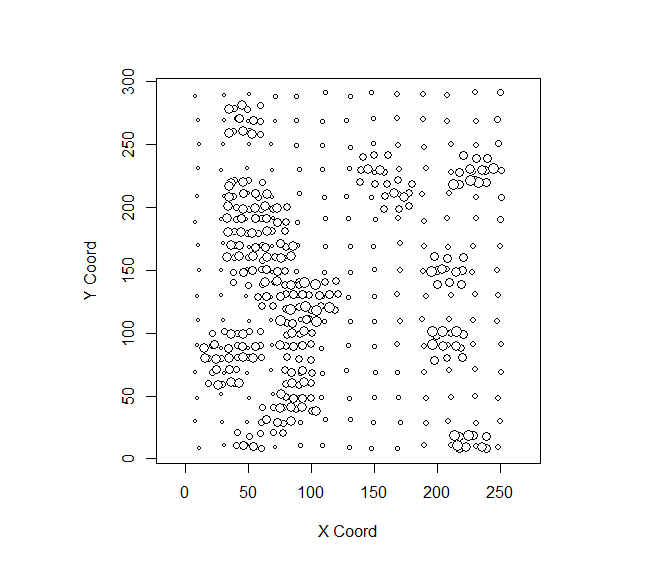
\includegraphics[scale=0.8]{Map_loc.png}	
	\caption{Mapa de localização das amostras do Walker Lake}
	\label{walk}
\end{figure}
\FloatBarrier

Outro gráfico com excelente visualização dos valores das variáveis pode ser realizado com o ssplot(). Mas antes para gerar os dados precisamos associar ao banco de dados do Walker Lake suas coordenadas. Para isso usamos o comando coordinates() e a ele associamos os valores das variáveis X e Y.


\begin{scriptsize}
	\estiloR
	\begin{lstlisting}[caption={Criação de um vetor em R}, label=lst:rcode]
	
	
	# ASSOCIAR AS COORDENADAS NO ESPACO
	coordinates(walker) = c("X", "Y")
	
	# SSPLOT DA VARIAVEL V 
	spplot(walker, c("V"),scales = list(draw =T))
	
	# SSPLOT DA VARIAVEL  V E U 
	spplot(walker, c("V","U"),scales = list(draw =T))
	
	\end{lstlisting}
\end{scriptsize}

A figura abaixo demonstra o mapa de intervalos para o depósito do Walker Lake. Os valores da variável V se alteram de 0 para 1528, e podemos notar que as regiões mais ricas se situam dentro do maior corpo do depósito na região oeste.

\FloatBarrier
 \begin{figure}[H]
	\centering
	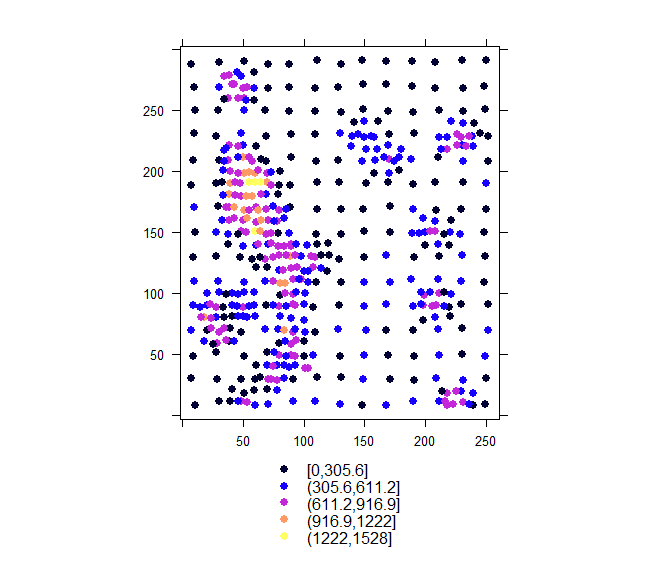
\includegraphics[scale=0.8]{Walker_points.png}	
	\caption{Mapa de intervalos das amostras do Walker Lake, variável V}
	\label{walk}
\end{figure}
\FloatBarrier

A Figura abaixo demonstra as variações para concumitantes para as variáveis V e U, dessa forma conseguimos visualizar a correlaçào entre as variáveis tal como o local onde foram amostradas. 

\FloatBarrier
 \begin{figure}[H]
	\centering
	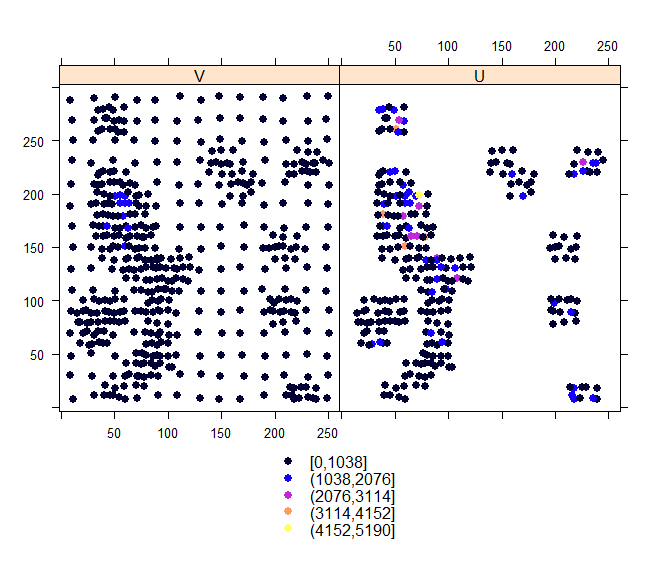
\includegraphics[scale=0.8]{Walker_points2.png}	
	\caption{Mapa de intervalos das amostras do Walker Lake, variável U e V}
	\label{walk}
\end{figure}
\FloatBarrier


\section{Histogramas} 

Podemos gerar histogramas das variáveis de interesse utilizando a função hist(), sendo o primeiro argumento a variável utilizada na construção do gráfico. O número de classes pode ser selecionado de acordo com o argumento breaks. Os argumentos xlab, ylab e main apenas definem o nome dos eixos plotados no gráfico. O R permite a utilização de múltiplos gráficos na mesma figura, isso pode ser obtido utilizando o comando par, e fornecendo um vetor para o argumento mfrow com o número de linhas e de colunas, respectivamente.

\begin{scriptsize}
	\estiloR
	\begin{lstlisting}[caption={Criação de um vetor em R}, label=lst:rcode]
	
	
	# funcao para criar mais de um grafico junto 
	par(mfrow = c(1,2))
	
	# Adicionar grafico da variavel U
	hist(walker$U, main= "histograma da variavel U ", breaks =15, xlab= "U", ylab= "Frequencia")
	
	# Adicionar grafico da variavel V
	hist(walker$V, main= "histograma da variavel V", breaks = 15,  xlab= "V", ylab = "Frequencia")
	
	\end{lstlisting}
\end{scriptsize}

A figura abaixo demonstra os histogramas gerados pelo código fonte. Notamos uma alta assimetria na variável U, enquanto a variável V demonstra valores mais espaçados entre si. 

\FloatBarrier
\begin{figure}[h]
	\centering
	\includegraphics[scale=0.8]{hist_Walker.png}	
	\caption{Histogramas das variáveis U e V do Walker Lake}
	\label{walk}
\end{figure}
\FloatBarrier

\section{Boxplots} 

Gráficos de caixa, ou também chamados de "boxplot" são uma ferramenta importante para avaliação de valores outliers que podem distorcer as estatísticas. Muito cuidado deve ser tomado na hora do tratamento de valores anômalos. Se as distribuições forem altamente assimétricas o gráfico pode apresentar um número muito grande de valores anômalos falseados, sendo necessário cautela na remoção destes valores.  

\begin{scriptsize}
	\estiloR
	\begin{lstlisting}[caption={Criação de um vetor em R}, label=lst:rcode]
	
	
	par(mfrow = c(1,2))
	boxplot(walker$U, main= "Boxplot da variavel U ", ylab= "U")
	boxplot(walker$V, main= "Boxplot da variavel V",  ylab= "V")
	
	\end{lstlisting}
\end{scriptsize}

A figura abaixo demonstra o gráfico de caixas utilizado para a modelagem matemática do Walker Lake. Notamos que a variável U apresenta um ponto discrepante acima de 5000.

\FloatBarrier
\begin{figure}[h]
	\centering
	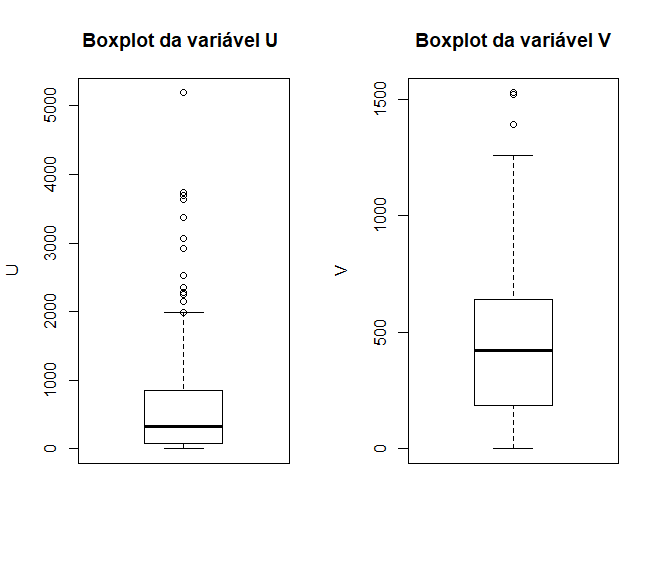
\includegraphics[scale=0.8]{box_walk.png}	
	\caption{Boxplot das variáveis U e V do Walker Lake}
	\label{walk}
\end{figure}
\FloatBarrier

\section{Regressão Linear}

Para realizarmos um modelo de regressão linear podemos utilizar o comando lm() em que primeiramente informamos a variável Y, e em seguida informamos a variável X separando-a por um sinal de \~. Para obtermos informações sobre os valores da regressão, basta utilizar a função summary, ao qual será informadas várias estatísticas, inclusive o coeficiente de regressão de Pearson. Em seguida para plotarmos o gráfico podemos utilizar a função plot, informando os valores de X e de Y. A reta de regressão pode ser adicionada utilizando o comando abline() e informando como argumento o modelo linear.

\begin{scriptsize}
	\estiloR
	\begin{lstlisting}[caption={Criação de um vetor em R}, label=lst:rcode]
	
	
	#Regressao Linear
	linear = lm(walker$U~walker$V)
	summary(linear)
	
	# Plotagem do resultado
	plot(walker$V, walker$U, xlab="V", ylab="U")
	abline(linear)
	
	\end{lstlisting}
\end{scriptsize}


O gráfico abaixo representa o modelo de regressão para as variáveis V e U. Um dos pontos acima do valor de 5000 parece demonstrar um valor outlier. 


\FloatBarrier
\begin{figure}[H]
	\centering
	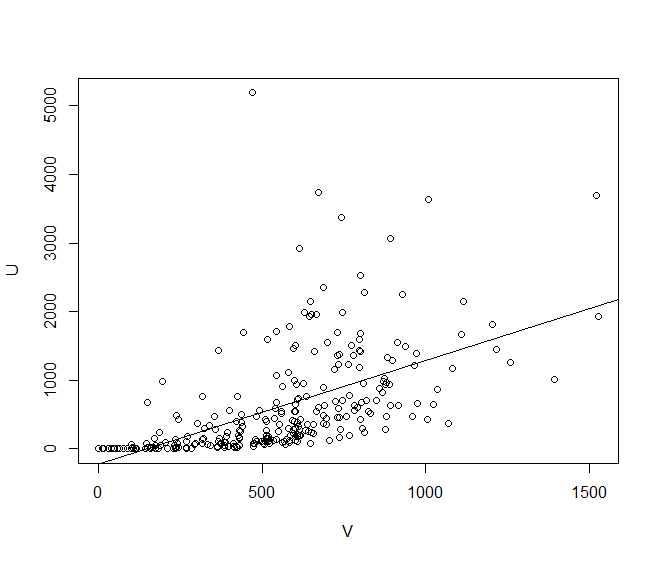
\includegraphics[scale=0.8]{regression_walker.png}	
	\caption{Regressão linear das variáveis U e V do Walker Lake}
	\label{walk}
\end{figure}
\FloatBarrier

\section{Vizinho mais próximo} 

Como metodologia para o desagrupamento, optamos por utilizar o vizinho mais próximo para encontrar as estatísticas desagrupadas. Primeiramente precisamos criar um grid, onde será realizada as interpolações. A função makegrid constrói um grid com um tamanho de célula definida pelo argumento cellsize. Para que possamos observar os resultados em um mapa de pixels, precisamos realizar algumas conversões, transformando primeiro em um objeto de pontos e em seguida de pixels. Em seguida podemos realizar a interpolação por vizinhos mais próximos, criando um raster dos dados e um objeto gstat que será utilizado na interpolação. Neste último definimos o número máximo de pontos considerados na interpolação do vizinho mais próximos. Ao atribuirmos nmax = 1 dizemos que cada valor da célula receberá única, e exclusivamente o valor da amostra mais próxima desta.

\begin{scriptsize}
	\estiloR
	\begin{lstlisting}[caption={Criação de um vetor em R}, label=lst:rcode]
	
	
	# Criar um grid 
	grid_stat = makegrid(walker,cellsize = 5)
	grid_stat = SpatialPixels(SpatialPoints(grid_stat))
	
	
	# Calcular vizinho mais proximo
	
	ca = raster(walker, res= 1)
	gs = gstat(NULL, "V", V~1, walker, nmax=1)
	nn = interpolate(ca, gs)
	plot(nn, axes=T)
	
	\end{lstlisting}
\end{scriptsize}

O resultado da interpolação pode ser compartilhado na figura abaixo. 

\FloatBarrier
\begin{figure}[H]
	\centering
	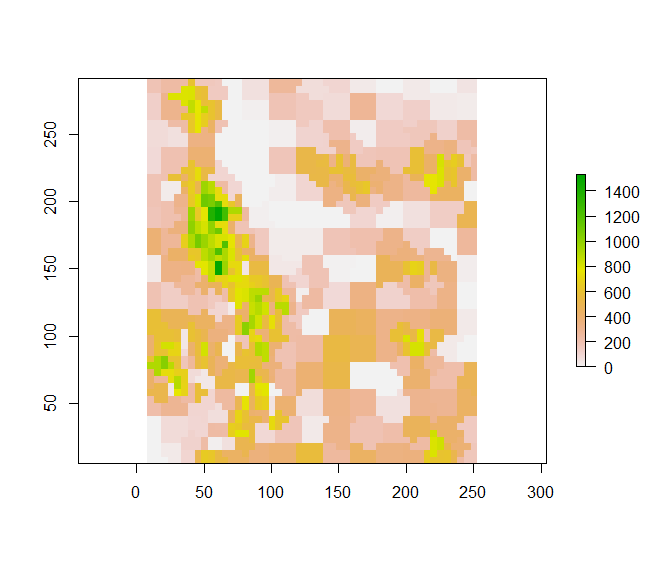
\includegraphics[scale=0.8]{nn_walk.png}	
	\caption{Vizinho mais próximo Walker Lake - variável V}
	\label{walk}
\end{figure}
\FloatBarrier

\section{Variograma} 

A variografia é uma das peças fundamentais para a criação de um modelo interpolado utilizando técnicas de geoestatística. Para avaliar a qualidade da dependência espacial dos dados, podemos utilizar uma ferramenta muito conhecida chamada de gráfico de dispersão h. Abaixo vemos o código fonte para a geração do gráfico. Primeiramente fornecemos o valor da variável a ser medida, em seguida o dataframe ao qual ela está contida e por fim o vetor com as distâncias para cada gráfico de dispersão.

\begin{scriptsize}
	\estiloR
	\begin{lstlisting}[caption={Criação de um vetor em R}, label=lst:rcode]
	
	# H-scatterplot da variavel V
	hscat(V~1, walker, (0:9)*5)
	
	\end{lstlisting}
\end{scriptsize}

A figura abaixo demonstra o gráfico de dispersão h para diferentes distâncias. Notamos que a correlação entre as variáveis distanciadas tende a cada vez mais decrescer de acordo com a distância entre os dados. 

\FloatBarrier
\begin{figure}[H]
	\centering
	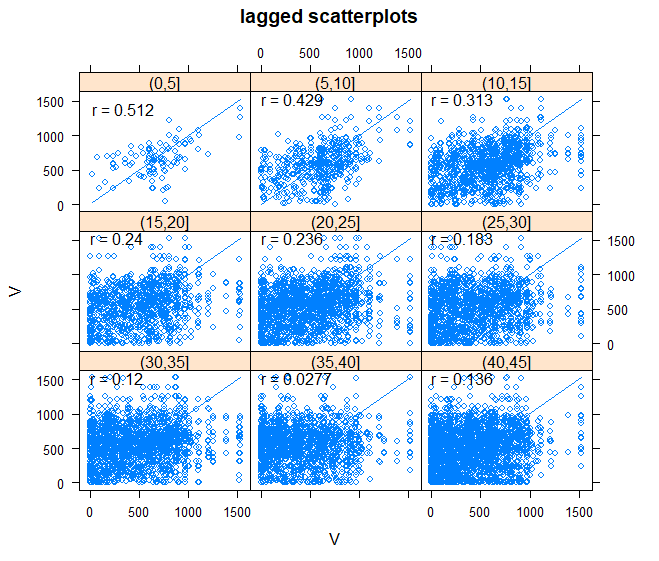
\includegraphics[scale=0.8]{hscat.png}	
	\caption{Hscatterplot para a variável V}
	\label{walk}
\end{figure}
\FloatBarrier

Variogramas são a principal ferramenta para a análise de continuidade espacial. Primeiramente
 precisamos saber a variância da variável modelada V, para que encontremos o valor máximo do patamar. Para isto utiilizamos o comando var(). Em seguida é necessário realizar o variograma experimental dos dados. Para isto utilizamos o comando variogram(). O primeiro argumento fornecido corresponde a variável utilizada. O segundo argumento corresponde ao dataframe considerado. O argumento width corresponde ao lag ou espaçamento utilizado para o cálculo dos variogramas experimentais. O cutoff representa a distância máxima para se calcular o variograma. Finalmente informamos a tolerância horizontal de cada um dos variogramas em graus. Como o problema é bidimensional, as direções de cada um dos variogramas é controlada apenas pelo azimute. O argumento alpha corresponde a uma lista de valores ao qual será calculado o variograma, para identificarmos a direção de máxima continuidade. 

\begin{scriptsize}
	\estiloR
	\begin{lstlisting}[caption={Criação de um vetor em R}, label=lst:rcode]
	
	
	#Variancia da variavel V
	var(walker$V)
	
	#Variogramas experimentais 
	
	v.dir = variogram(V~1, walker, width=10, cutoff= 200, tol.hor=45, alpha = (0:7)*22.5 )

	\end{lstlisting}
\end{scriptsize}

\FloatBarrier
\begin{figure}[H]
	\centering
	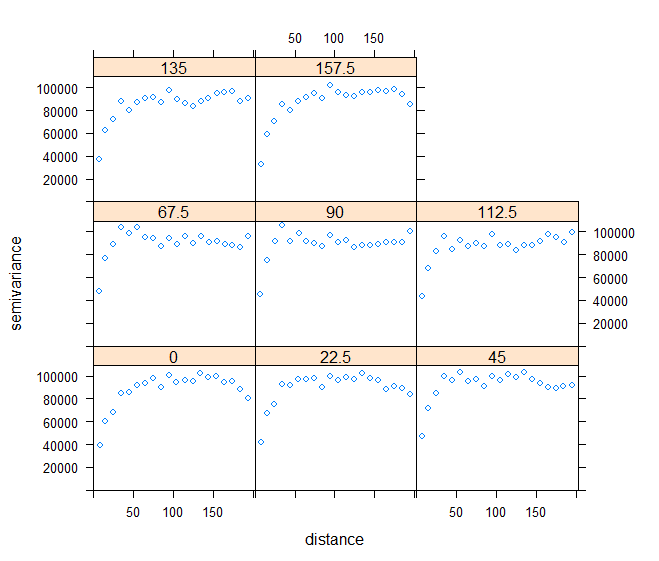
\includegraphics[scale=0.9]{var_experimentais.png}	
	\caption{Variogramas experimentais gerados}
	\label{walk}
\end{figure}
\FloatBarrier

A modelagem de variogramas individuais pode ser realizada a partir da biblioteca geoR utilizando o comando eyefit. para isso criamos um objeto do variograma experimental utilizando a função variog() e atribuímos os argummentos relacionados com o variograma, tais como direção (em radianos), tolerância angular (em radianos), o argumento uvec, que representa o vetor com distâncias a serem calculadas e a máxima distância de cáculo. Lembre-se que para utilizar as rotinas do pacote geoR é necessário transformar o banco de dados em um tipo específico chamado de geodata. 



\begin{scriptsize}
	\estiloR
	\begin{lstlisting}[caption={Criação de um vetor em R}, label=lst:rcode]
	
	
	library(geoR)
	library(gstat)
	
	# Baixar os dados do Walker Lake
	data(walker)
	
	# Associar coordenadas ao banco de dados 
	coordinates(walker) = c('X', 'Y')
	
	#Criar variograma experimental utilizando a biblioteca geoR
	var = variog(as.geodata(walker["V"]), uvec = seq(from=0,to=500,by=10),max.dist = 500, direction= 157.5*pi/180, tolerance = pi/4)
	
	#Fitar manualmente o variograma  
	ve.eye = eyefit(var)
	
	#Transformar o modelo fitado em um modelo do gstat
	ve.fit = as.vgm.variomodel(v.eye[[1]])
	
	\end{lstlisting}
\end{scriptsize}

A figura abaixo demonstra o ajuste do modelo de variograma utilizando a função eyefit. Uma janela é aberta podendo ser selecionado os modelos mais adequados para o ajuste, tal como é possível também selecionar os melhores parâmetros como patamar, alcance e efeito pepita.

\FloatBarrier
\begin{figure}[H]
	\centering
	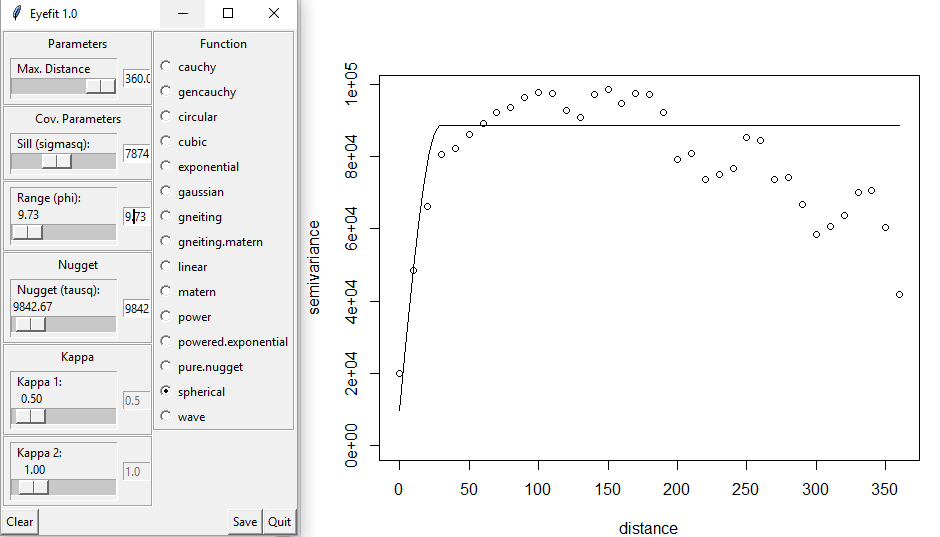
\includegraphics[scale=0.6]{eyefit.png}	
	\caption{Ajuste do modelo de variograma utilizando a função eyefit}
	\label{walk}
\end{figure}
\FloatBarrier

Para ajustarmos um modelo de variograma podemos utilizar a função vgm() para as diferentes direções e para diferentes estruturas. Diversos são os tipos de modelos aceitados pela função. A tabela abaixo demonstra uma relação dos modelos abordados pela função vgm.  

\FloatBarrier
\begin{table}[h]
	\centering
	\begin{tabular}{@{}lll@{}}
		\toprule
		& Forma curta & Forma longa \\ \midrule
		1 & Nug & Nug (nugget) \\
		2 & Exp & Exp (exponential) \\
		3 & Sph & Sph (spherical) \\
		4 & Gau & Gau (gaussian) \\
		5 & Exc & \begin{tabular}[c]{@{}l@{}}Exclass\\   (Exponential class/stable)\end{tabular} \\
		6 & Mat & Mat (Matern) \\
		7 & Ste & \begin{tabular}[c]{@{}l@{}}Mat (Matern M. Stein's\\   parameterization)\end{tabular} \\
		8 & Cir & Cir (circular) \\
		9 & Lin & Lin (linear) \\
		10 & Bes & Bes (bessel) \\
		11 & Pen & Pen (pentaspherical) \\
		12 & Per & Per (periodic) \\
		13 & Wav & Wav (wave) \\
		14 & Hol & Hol (hole) \\
		15 & Log & Log (logarithmic) \\
		16 & Pow & Pow (power) \\
		17 & Spl & Spl (spline) \\
		18 & Leg & Leg (Legendre) \\
		19 & Err & \begin{tabular}[c]{@{}l@{}}Err\\   (Measurement error)\end{tabular} \\
		20 & Int & Int (Intercept) \\ \bottomrule
	\end{tabular}
	\caption{Modelos permissíveis de variograma para o objeto vgm}
	\label{tab:my-table}
\end{table}
\FloatBarrier

Para utilizarmos a função vgm() primeiramente adicionamos como argumento inicial a contribuição da estrutura, o tipo de modelo (Esférico, Exponencial, etc), o alcance da estrutura e o efeito pepita. Podemos adicionar o parâmetro anis, ao qual contém primeiramente o azimute (em graus) da direção principal e o fator de redução do alcance para a elipse. Em outras palavras se o alcance máximo na direção principal é 50m, ao adicionarmos um fator de 0.6 fazemos com que a direção de menor continuidade seja de 30m. Para adicionarmos mais de uma estrutura podemos concatená-las com o argumento add.to, adicionando quantas estruturas forem necessárias para formar o modelo de continuidade espacial. Finalmente podemos plotar o gráfico utilizando o comando plot(). O código fonte abaixo demonstra como obter um modelo de variograma a partir dos dados do Walker Lake.

\begin{scriptsize}
	\estiloR
	\begin{lstlisting}[caption={Criação de um vetor em R}, label=lst:rcode]
	
	
	#Variancia da variavel V
	var(walker$V)
	
	#Variogramas experimentais
	
	v.dir = variogram(V~1, walker, width=10, cutoff= 200, tol.hor=45, alpha = (0:7)*22.5 )
	
	# Modelagem da primeira estrutura 
	
	v.anis1 = vgm(59929,"Sph",40,20000, anis=c(157,0.6))
	
	# Modelagem da segunda estrutura 
	
	v.anis2 = vgm(20000,"Exp",100, 0, anis=c(157,0.6),add.to =v.anis1 )
	
	# Plotagem do grafico
	plot(v.dir, v.anis2)
	
	\end{lstlisting}
\end{scriptsize}

A figura abaixo demonstra o modelo de continuidade espacial para o Walker Lake para a variável V. Neste caso a direção de maior continuidade foi considerada em 157.5 graus e duas estruturas foram adicionadas. 

\FloatBarrier
\begin{figure}[H]
	\centering
	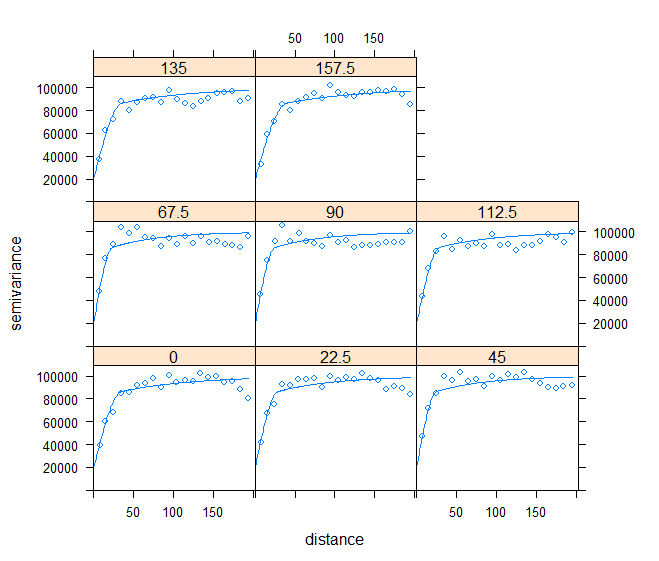
\includegraphics[scale=0.9]{walker_model.png}	
	\caption{Ajuste do modelo para diferentes direções utilizando a função vgm}
	\label{walk}
\end{figure}
\FloatBarrier


\section{Validação Cruzada} 

Para testar a eficiência de diferentes modelos de variograma, tal como diferentes estratégias de busca da krigagem, podemos utilizar a validação cruzada. De acordo com os erros exibidos pela validação, podemos modificar os parâmetros de krigagem e do variograma para obter os menores erros possíveis. O resíduo é uma medida adequada neste caso para o erro de estimativa, podemos plotar os resultados em um gráfico de bolhas. A função krige.cv() é calculada fornecendo primeiramente a variável de interesse, o dataframe que está contido a variável, o modelo de variograma ajustado na seção anterior, o número mínimo de amostras utilizadas na krigagem, o número máximo de amostras utilizadas na krigagem, a máxima distância de procura dos dados e o número de dados retirados durante a validação para se computar o erro médio dos valores reais e krigados. O código fonte abaixo demonstra a validação cruzada.  

\begin{scriptsize}
	\estiloR
	\begin{lstlisting}[caption={Criação de um vetor em R}, label=lst:rcode]
	
	# Validacao cruzada
	cv = krige.cv(V~1, walker, v.anis2 , nmin= 3, nmax=10, maxdist=100, nfold=20)
	
	# Sumario estatistico da validacao
	summary(cv)
	
	#Plotagem dos residuos da validacao cruzada
	bubble(cv["residual"])
	
	\end{lstlisting}
\end{scriptsize}

A figura abaixo demonstra os erros residuais a partir da validação cruzada do depósito Walker Lake. 

\FloatBarrier
\begin{figure}[H]
	\centering
	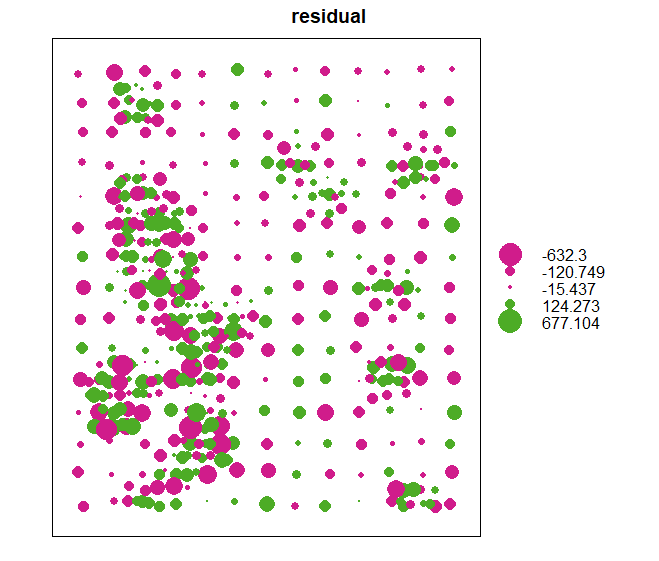
\includegraphics[scale=0.8]{bubble.png}	
	\caption{Erros da validação cruzada demonstrados em um gráfico de bolhas}
	\label{walk}
\end{figure}
\FloatBarrier

\section{Krigagem} 

Encontrados os melhores modelos de variograma e estratégia de busca possíveis, podemos realizar a krigagem da variável de interesse V. Para isso criamos um grid assim como no vizinho mais próximo utilizando os comandos já conhecidos. Então utilizamos o comando krige(), cujos argumentos são, primeiramente a variável de interesse a ser krigada, em seguida o dataframe em que esta variável está contida, o grid criado e os parâmetros da estratégia de busca, tais como mínimo número de amostras (nmin), máximo número de amostras (nmax), a máxima distância de procura (nmax) e finalmente o modelo de variograma ajustado. O código fonte abaixo demonstra a krigagem dos valores da variável V, do depósito do Walker Lake. 


\begin{scriptsize}
	\estiloR
	\begin{lstlisting}[caption={Criação de um vetor em R}, label=lst:rcode]
	
	# Criar um grid 
	grid_stat = makegrid(walker,cellsize = 5)
	grid_stat = SpatialPixels(SpatialPoints(grid_stat))
		
	# Krigar os valores
	kriged = krige(V~1, walker, grid_stat,nmin=2, nmax=3, maxdist=100, v.anis2)
	
	# Plotar a variavel estimada
	spplot(kriged['var1.pred'], scales = list(draw =T))
	
	# Plotar a variancia de krigagem
	spplot(kriged['var1.var'] , scales = list(draw =T))
	summary(kriged)
	
	\end{lstlisting}
\end{scriptsize}

O gráfico abaixo demonstra o valor krigado da variável V a partir da estratégia de busca e do variograma ajustado.

\FloatBarrier
\begin{figure}[H]
	\centering
	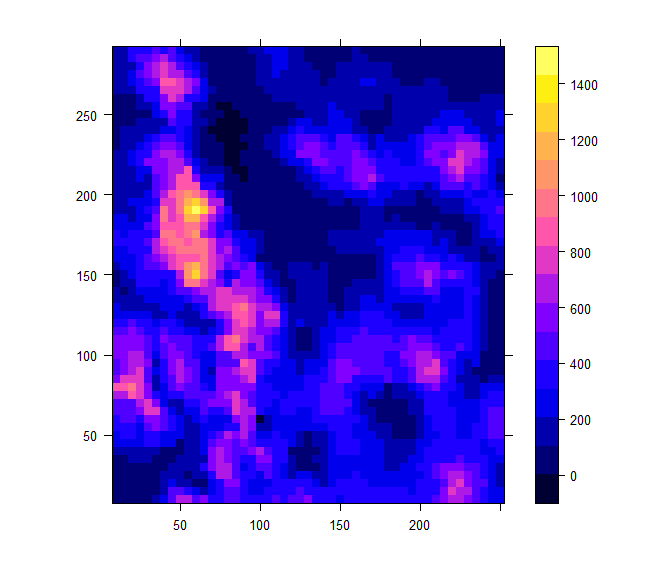
\includegraphics[scale=0.6]{walker_krig.png}	
	\caption{Krigagem da variável V do depósito Walker Lake}
	\label{walk}
\end{figure}
\FloatBarrier

O gráfico abaixo demonstra a variância de krigagem da variável V a partir da estratégia de busca e do variograma ajustado.

\FloatBarrier
\begin{figure}[H]
	\centering
	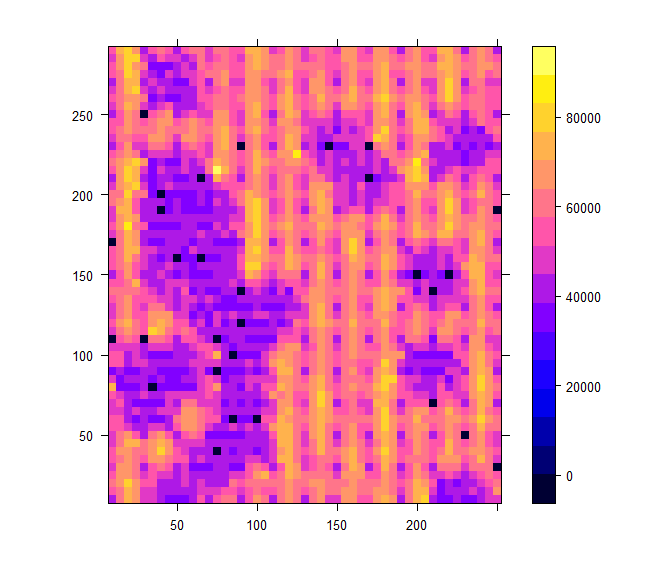
\includegraphics[scale=0.6]{walker_var_krig.png}	
	\caption{Krigagem da variável V do depósito Walker Lake}
	\label{walk}
\end{figure}
\FloatBarrier
